%%%%%%%%%%%%%%%%%%%%%%%%%%%%%%%%%%%%%%%%%%%%%%%%%%%%%%%%%%%%%%%%%%%%%%%%%%%%%%%
%                                                                             %
%    DOCUMENTO LATEX - HEADER                                                 %
%                                                                             %
%%%%%%%%%%%%%%%%%%%%%%%%%%%%%%%%%%%%%%%%%%%%%%%%%%%%%%%%%%%%%%%%%%%%%%%%%%%%%%%

%escolha uma  classe

\documentclass[notes, mathserif]{beamer}
\beamertemplateshadingbackground{gray!20}{white!10}

% Pacotes
\usepackage{pgf,pgfarrows,pgfnodes,pgfautomata,pgfheaps,pgfshade}
\usepackage{amsmath,amssymb}
\usepackage{colortbl}
\usepackage[latin1]{inputenc}
\usepackage[brazil]{babel}
\usepackage{mathtools}
\usepackage{xlop}
\usepackage{diagbox}
\usepackage[linesnumbered,ruled]{algorithm2e}
\beamertemplatetransparentcovereddynamic
\beamertemplatenavigationsymbolsempty

% Comandos
%\setlength{\belowcaptionskip}{0cm}

\DeclarePairedDelimiter{\ceil}{\lceil}{\rceil}%

\setbeamercovered{highly dynamic}
\newcounter{saveenumi}
\newcommand{\seti}{\setcounter{saveenumi}{\value{enumi}}}
\newcommand{\conti}{\setcounter{enumi}{\value{saveenumi}}}
\resetcounteronoverlays{saveenumi}
% Tema
\usetheme{Luebeck}
\useinnertheme{rectangles}

% Informa  o
\title[Porte do jogo \textit{Traveling Will} para GBA]
{Porte do jogo \textit{Traveling Will} para o \textit{Nintendo Game Boy Advance}}
\subject{}
\institute{Faculdade Gama
\\ Universidade de Bras\'ilia\\ Brasil}
\date{10 de dezembro de 2018}
\author[Igor Duarte e V\'itor Barbosa]
{
  Igor Ribeiro Barbosa Duarte e V\'itor Barbosa de Araujo
}

 \begin{document}
 \frame{\titlepage}
%\frame{\frametitle{Sum�rio}\tableofcontents[pausesections]}

\begin{frame}{Objetivo geral}
	\begin{itemize}[<+->]
		\item O objetivo geral deste trabalho \'e reescrever o jogo \textit{Traveling Will}, desenvolvido originalmente para PC na disciplina de Introdu\c c\~ao aos Jogos Eletr\^onicos, para o \textit{Nintendo Game Boy Advance}
	\end{itemize}
\end{frame}

\begin{frame}{Objetivos espec\'ificos}
	Os objetivos espec\'ificos s\~ao:
	\begin{itemize}[<+->]
		\item Comprimir imagens e m\'usicas do jogo original para reduzir o uso de mem\'oria;
		\item Criar m\'odulos para renderiza\c c\~ao de imagens e texto;
		\item Criar m\'odulos para manipula\c c\~ao de \textit{inputs} dos bot\~oes e carregamento de \'audio;
		\item Criar m\'odulos para detec\c c\~ao de colis\~oes e manipula\c c\~ao de eventos;
		\item Criar m\'etodos para carregamento do \textit{level design} das fases do jogo;
		\item Executar e testar o jogo desenvolvido na plataforma escolhida.
	\end{itemize}
\end{frame}

\section{Metodologia}

\begin{frame}{Ferramentas}
	Para o porte do jogo foram utilizadas as seguintes ferramentas:

		\begin{itemize}[<+->]
			\item \textit{C++}
			\item \textit{devkitARM}
			\item \textit{GIMP}
			\item \textit{GRIT}
			\item \texttt{avconv, librosa} e \texttt{modplug tracker}
			\item \textit{VisualBoyAdvance-M}
			\item \textit{Nintendo DS}
			\item \textit{EZFlash II}
		\end{itemize}
\end{frame}


\begin{frame}{Desenvolvimento da \textit{engine}}
	Para este trabalho foi desenvolvida a \texttt{gbengine}.
	\begin{itemize}[<+->]
		\item M\'odulos implementados: \textit{input}, v\'ideo, gerenciador de mem\'oria, \'audio e f\'isica;
		\item \textbf{M\'odulo de \textit{input}}: detectar pressionamento dos bot\~oes do GBA.
		\item \textbf{M\'odulo de v\'ideo}: renderizar, animar e atualizar imagens;
		\item \textbf{M\'odulo gerenciador de mem\'oria}: garantir aloca\c c\~ao segura e eficiente de mem\'oria;
		\item \textbf{M\'odulo de \'audio}: iniciar e parar m\'usicas de fundo;
		\item \textbf{M\'odulo de f\'isica}: simular a a\c c\~ao de gravidade e detectar colis\~oes entre objetos do jogo;
	\end{itemize}
\end{frame}

\section{Resultados - Desenvolvimento da engine}

\begin{frame}{M\'odulo de input}
	\begin{itemize}
		\item Detectar pressionamento dos bot\~oes
		\item \textit{Bitmask} onde o valor \texttt{0} indica pressionamento
	\end{itemize}
\end{frame}

\begin{frame}{M\'odulo de input}
	\begin{figure}[H]
		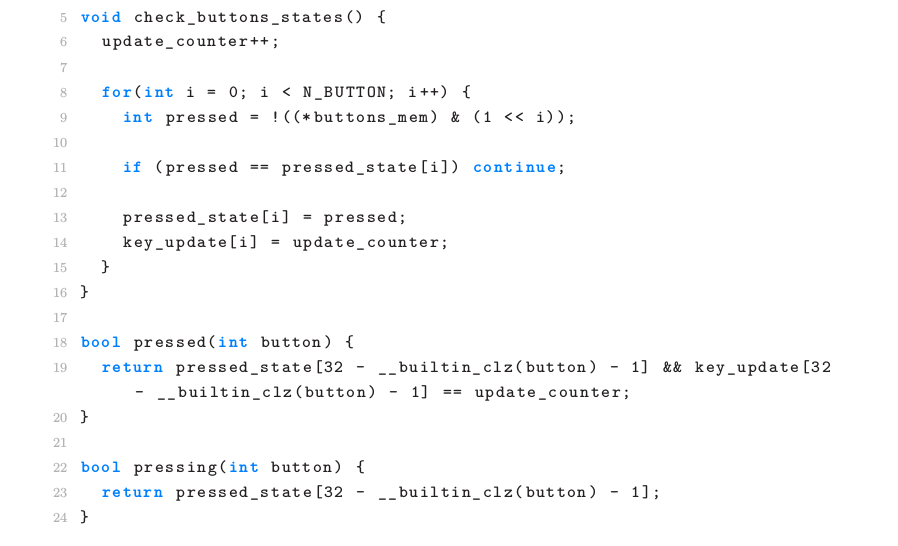
\includegraphics[width=1\linewidth]{figuras/input-codigo.png}
		\centering
		\caption{C\'odigo da classe \textit{input}}
		\label{fig:inputcode}
	\end{figure}
\end{frame}

\begin{frame}{M\'odulo de input}
	\begin{figure}[H]
		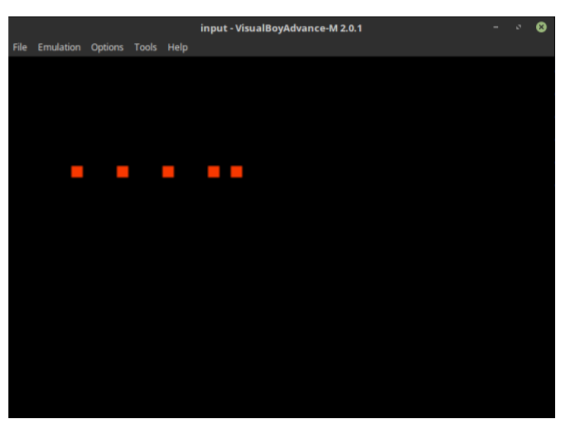
\includegraphics[width=.7\linewidth]{figuras/input-demo.png}
		\centering
		\caption{\textit{Demo} do \textit{input}}
		\label{fig:inputdemo}
	\end{figure}
\end{frame}

\begin{frame}{M\'odulo de input}
	\begin{figure}[H]
		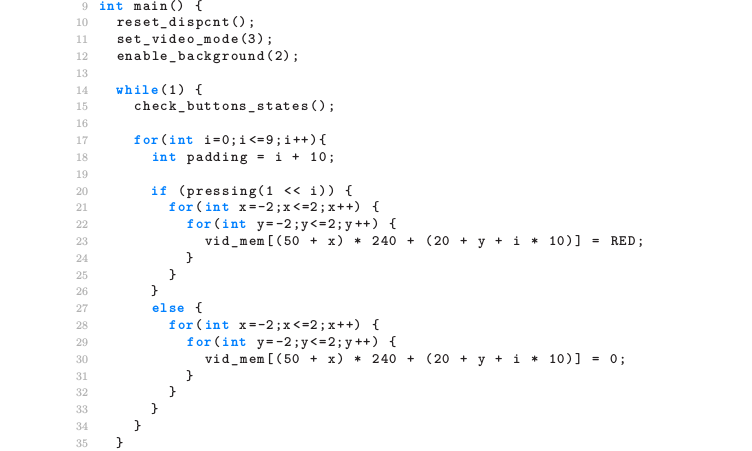
\includegraphics[width=.9\linewidth]{figuras/input-demo-codigo.png}
		\centering
		\caption{C\'odigo do \textit{demo} de \textit{input}}
		\label{fig:inputdemocode}
	\end{figure}
\end{frame}

\begin{frame}{M\'odulo de v\'ideo}
\end{frame}

\begin{frame}{M\'odulo gerenciador de mem\'oria}
	\begin{itemize}
		\item Garantir aloca\c c\~ao segura e eficiente de mem\'oria
		\item Gerenciamento com parti\c c\~oes vari\'aveis
	\end{itemize}
\end{frame}

\begin{frame}{M\'odulo gerenciador de mem\'oria}
	Funcionamento do gerenciador de mem\'oria:
	\begin{itemize}
		\item Inicializar os ponteiros para as regi\~oes de mem\'oria
		\item Quando h\'a chamada de aloca\c c\~ao, procura pelo primeiro espa\c co dispon\'ivel
		\item Verificar espa\c co dispon\'ivel
		\item Liga posi\c c\~ao no \texttt{bitset}
		\item Retorna o ponteiro encontrado
	\end{itemize}
\end{frame}

\begin{frame}{M\'odulo gerenciador de mem\'oria}
	\begin{figure}[H]
		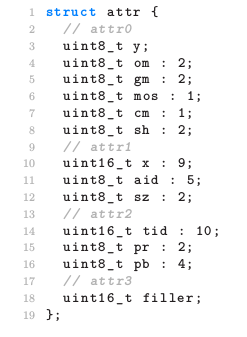
\includegraphics[width=.4\linewidth]{figuras/bitfield.png}
		\centering
		\caption{Uso de \textit{bitfields} nos metadados das \textit{sprites}}
		\label{fig:bitfield}
	\end{figure}
\end{frame}

\begin{frame}{M\'odulo gerenciador de mem\'oria}
	\begin{figure}[H]
		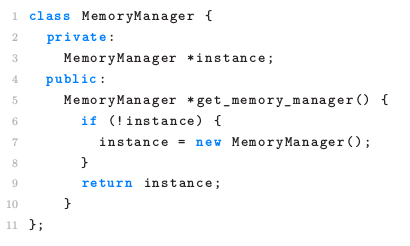
\includegraphics[width=.7\linewidth]{figuras/singleton.png}
		\centering
		\caption{Uso de \textit{singleton} na classe \texttt{MemoryManager}}
		\label{fig:singleton}
	\end{figure}
\end{frame}

\begin{frame}{M\'odulo de f\'isica}
	\begin{itemize}
		\item Checar se os objetos est\~ao colidindo
		\item Chamar \texttt{on\_collision()} do alvo
	\end{itemize}
\end{frame}

\begin{frame}{M\'odulo utilit\'ario}
	C\'odigo \textit{assembly} com chamada para \texttt{vbaprint()}
	\begin{figure}[H]
		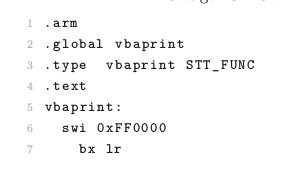
\includegraphics[width=.4\linewidth]{figuras/print_asm.png}
		\centering
		\caption{Chamada para \texttt{vbaprint()}}
		\label{fig:vbaprint}
	\end{figure}
\end{frame}


\begin{frame}{M\'odulo utilit\'ario}
	Fun\c c\~ao \texttt{print()}
	\begin{figure}[H]
		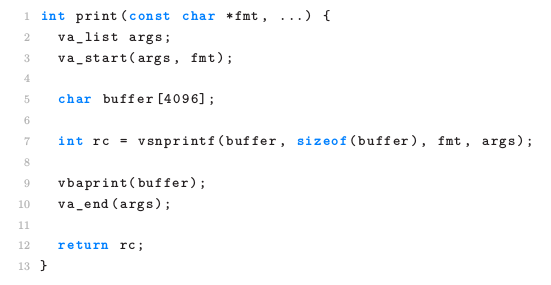
\includegraphics[width=.7\linewidth]{figuras/print.png}
		\centering
		\caption{Fun\c c\~ao \texttt{print()}}
		\label{fig:print}
	\end{figure}
\end{frame}

\begin{frame}{M\'odulo utilit\'ario}
	Fun\c c\~ao \texttt{mem16cpy()}
	\begin{figure}[H]
		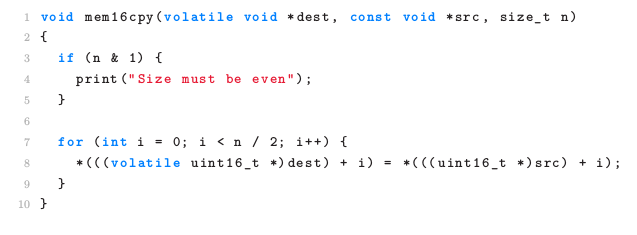
\includegraphics[width=.7\linewidth]{figuras/mem16cpy.png}
		\centering
		\caption{Fun\c c\~ao \texttt{mem16cpy()}}
		\label{fig:mem16cpy}
	\end{figure}
\end{frame}

\begin{frame}{M\'odulo utilit\'ario}
	Fun\c c\~ao \texttt{vsync()}
	\begin{figure}[H]
		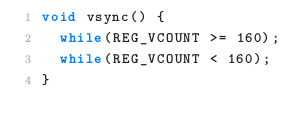
\includegraphics[width=.5\linewidth]{figuras/vsync.png}
		\centering
		\caption{Fun\c c\~ao \texttt{vsync()}}
		\label{fig:vsync}
	\end{figure}
\end{frame}

\section{Resultados - Desenvolvimento do jogo}

\begin{frame}{Adapta\c c\~ao das m\'usicas do jogo}
\end{frame}

\begin{frame}{Adapta\c c\~ao das imagens do jogo}
\end{frame}

\begin{frame}{Constru\c c\~ao dos n\'iveis do jogo}
	\begin{itemize}[<+->]
		\item \textit{Parser} para \textit{level design} original
		\item Reutilizar texturas das plataformas
		\item Carregar somente os itens vis\'iveis
	\end{itemize}
\end{frame}

\begin{frame}{Constru\c c\~ao dos n\'iveis do jogo}
	\begin{figure}[H]
		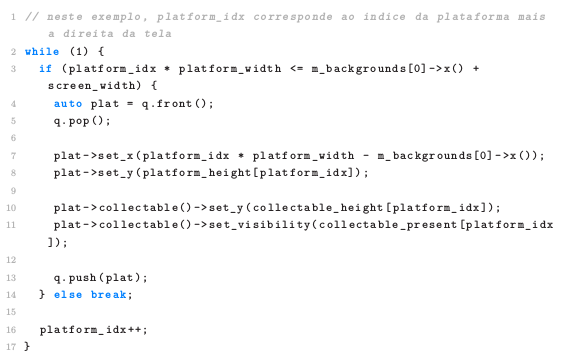
\includegraphics[width=.7\linewidth]{figuras/plats.png}
		\centering
		\caption{C\'odigo para atualiza\c c\~ao das plataformas}
		\label{fig:vsync}
	\end{figure}
\end{frame}

\begin{frame}{Transi\c c\~ao entre os n\'iveis do jogo}
	\begin{figure}[H]
		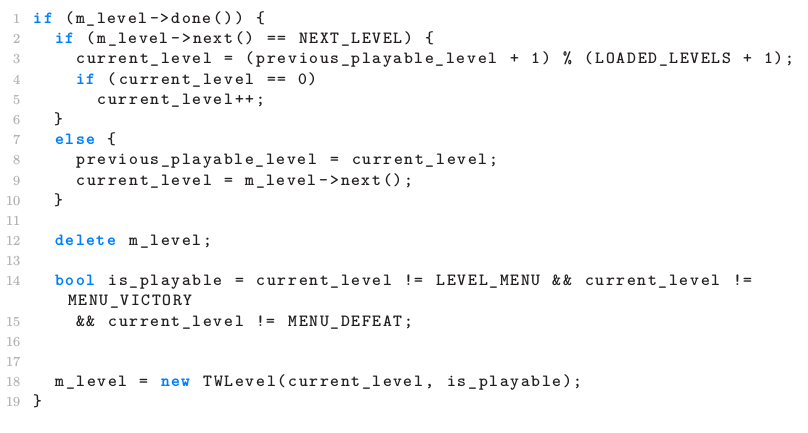
\includegraphics[width=.8\linewidth]{figuras/transicao.png}
		\centering
		\caption{Transi\c c\~ao entre n\'iveis}
		\label{fig:vsync}
	\end{figure}
\end{frame}

\begin{frame}{Classes do jogo}
	\begin{figure}[H]
		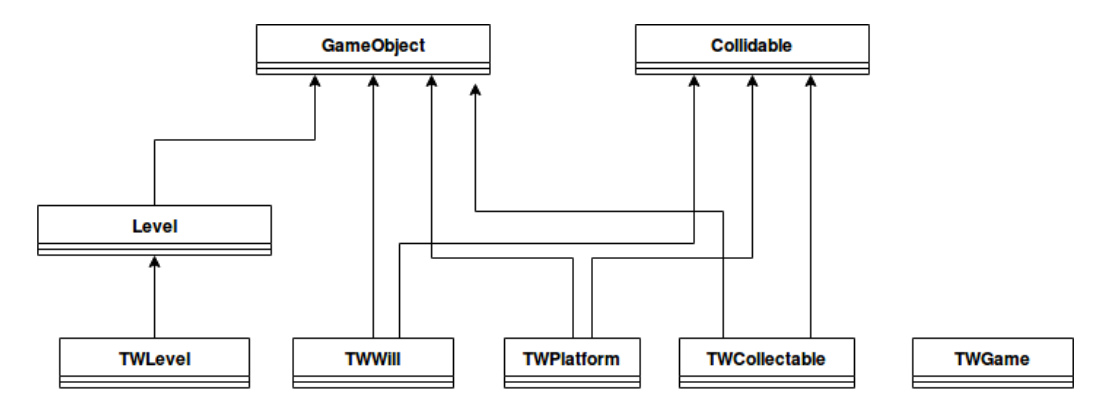
\includegraphics[width=1\linewidth]{figuras/classes.png}
		\centering
		\caption{Diagrama de classes do jogo.}
		\label{fig:vsync}
	\end{figure}
\end{frame}

\begin{frame}{Compara\c c\~ao entre o porte e o jogo original}
	\begin{figure}%
    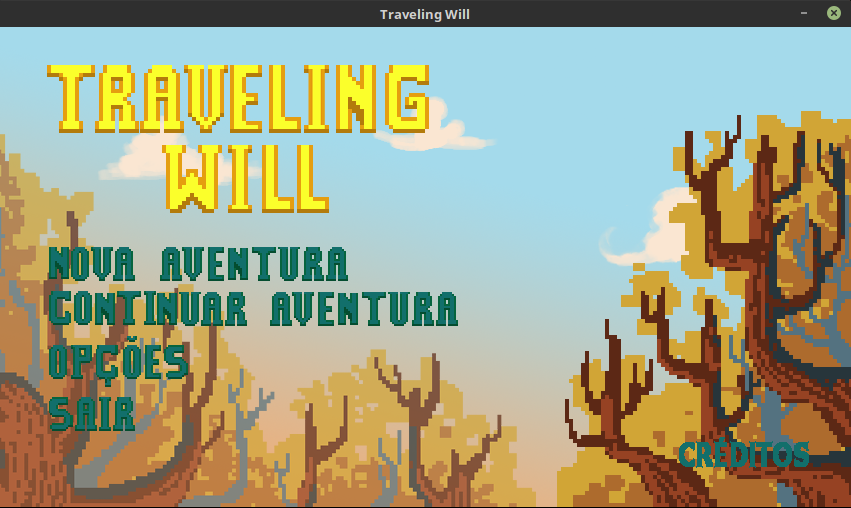
\includegraphics[width=.5\linewidth]{figuras/pc-menu.png}
    \qquad
    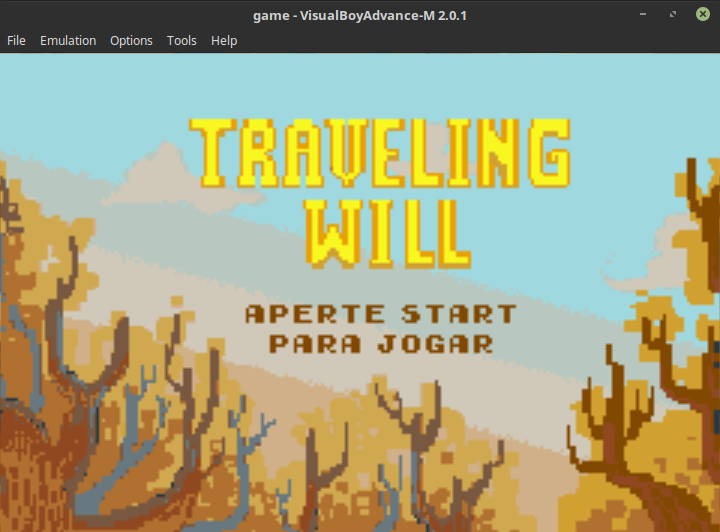
\includegraphics[width=.4\linewidth]{figuras/gba-menu.png}
    \caption{Compara\c c\~ao entre os menus.}%
    \label{fig:comp1}%
	\end{figure}
\end{frame}

\begin{frame}{Compara\c c\~ao entre o porte e o jogo original}
	\begin{figure}%
    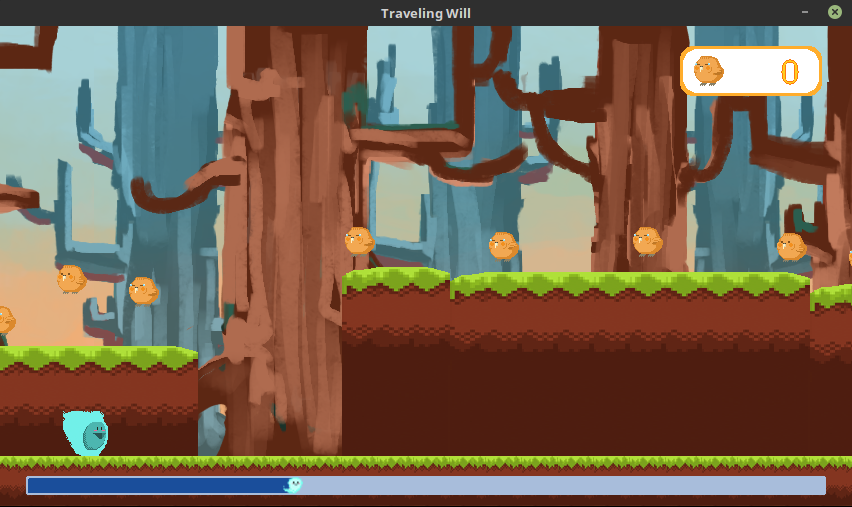
\includegraphics[width=.5\linewidth]{figuras/pc-fase1.png}
    \qquad
    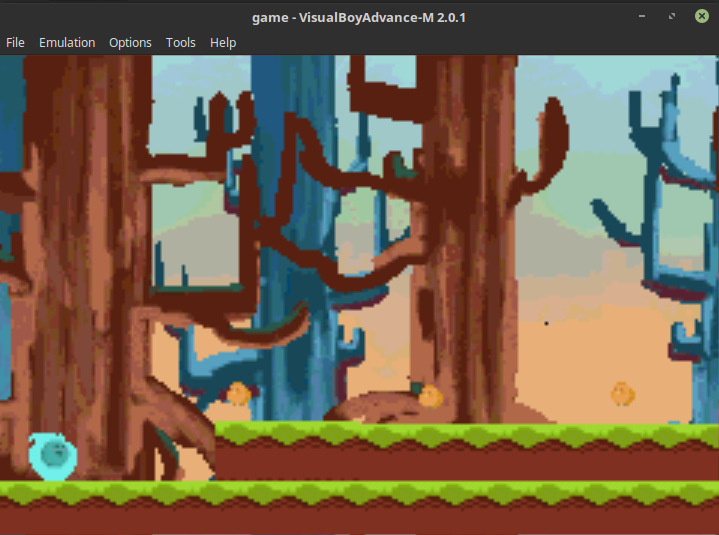
\includegraphics[width=.4\linewidth]{figuras/gba-fase1.png}
    \caption{Compara\c c\~ao da primeira fase.}%
    \label{fig:comp1}%
	\end{figure}
\end{frame}

\begin{frame}{Compara\c c\~ao entre o porte e o jogo original}
	\begin{figure}%
    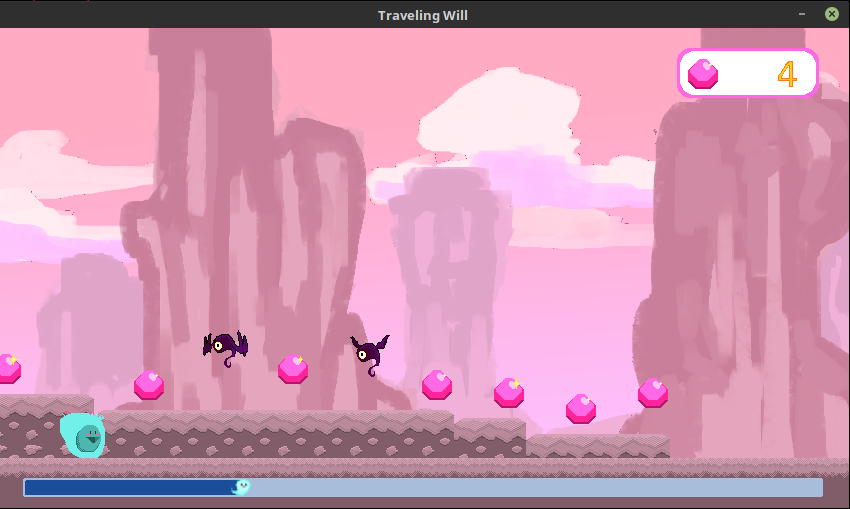
\includegraphics[width=.5\linewidth]{figuras/pc-fase2.png}
    \qquad
    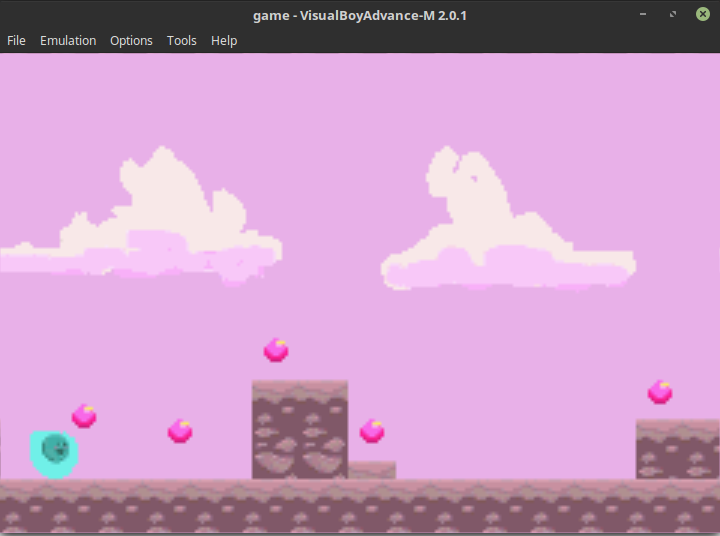
\includegraphics[width=.4\linewidth]{figuras/gba-fase2.png}
    \caption{Compara\c c\~ao da segunda fase.}%
    \label{fig:comp1}%
	\end{figure}
\end{frame}

\begin{frame}{Compara\c c\~ao entre o porte e o jogo original}
	\begin{figure}%
    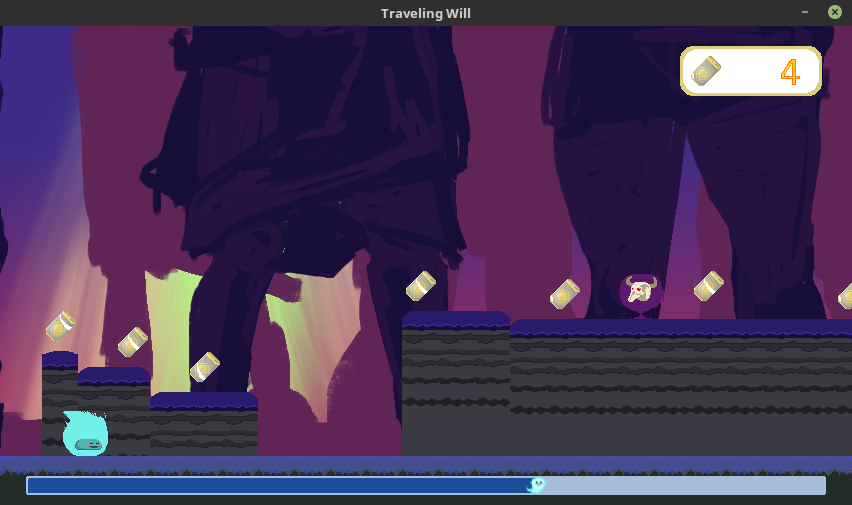
\includegraphics[width=.5\linewidth]{figuras/pc-fase3.png}
    \qquad
    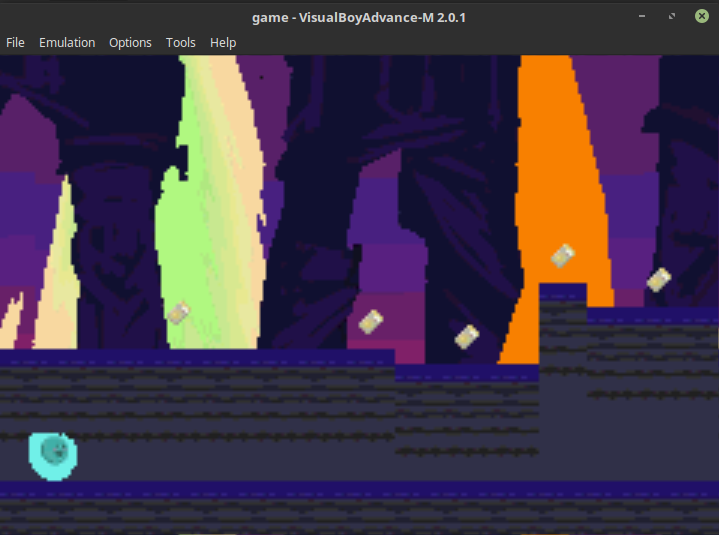
\includegraphics[width=.4\linewidth]{figuras/gba-fase3.png}
    \caption{Compara\c c\~ao da terceira fase.}%
    \label{fig:comp1}%
	\end{figure}
\end{frame}

\begin{frame}{Compara\c c\~ao entre o porte e o jogo original}
	\begin{figure}%
    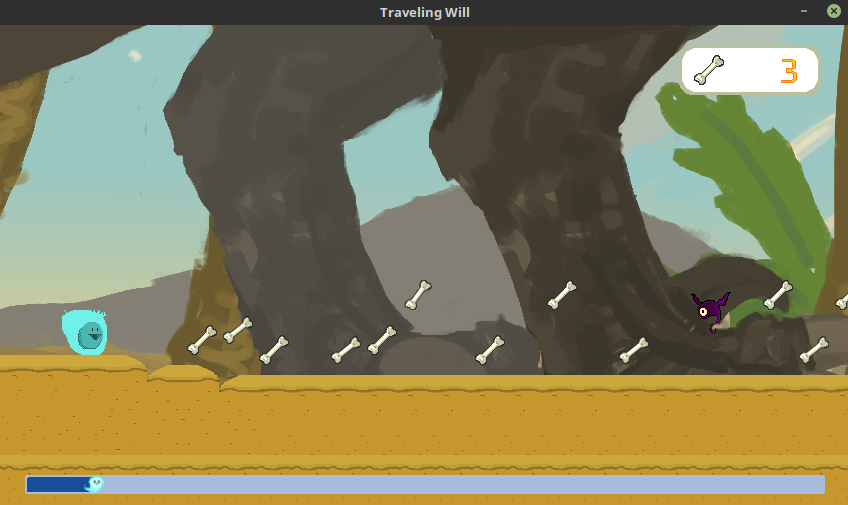
\includegraphics[width=.5\linewidth]{figuras/pc-fase4.png}
    \qquad
    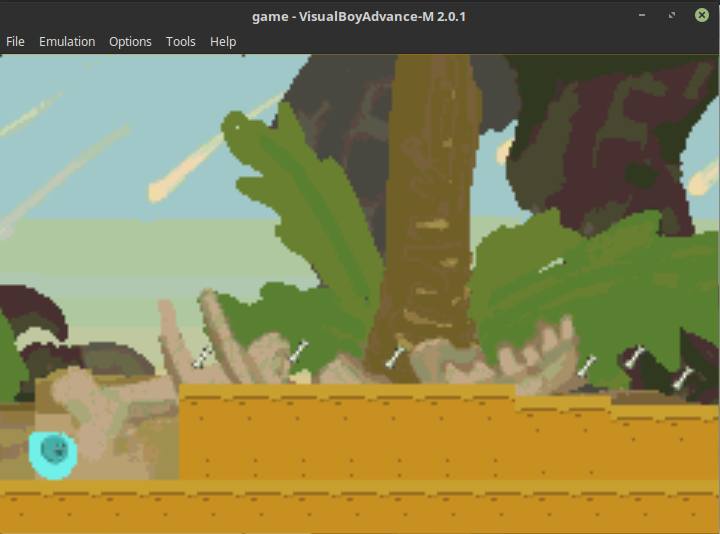
\includegraphics[width=.4\linewidth]{figuras/gba-fase4.png}
    \caption{Compara\c c\~ao da quarta fase.}%
    \label{fig:comp1}%
	\end{figure}
\end{frame}

\begin{frame}{Compara\c c\~ao entre o porte e o jogo original}
	\begin{figure}%
    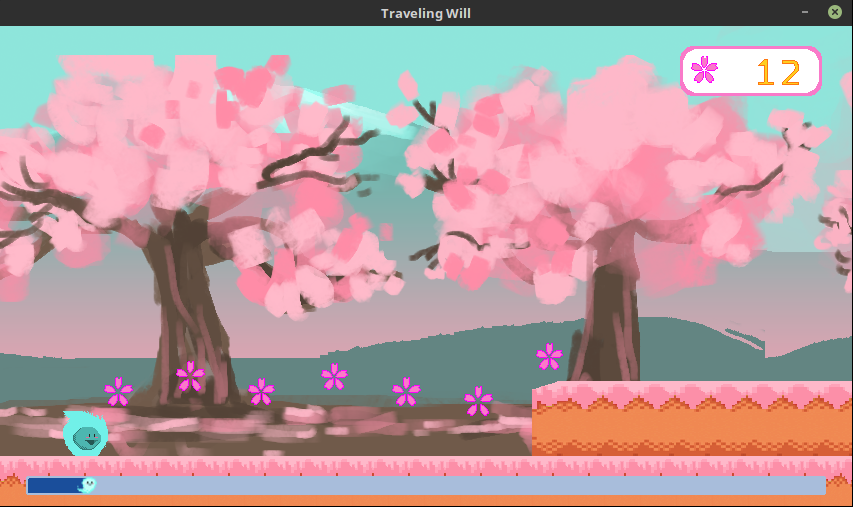
\includegraphics[width=.5\linewidth]{figuras/pc-fase5.png}
    \qquad
    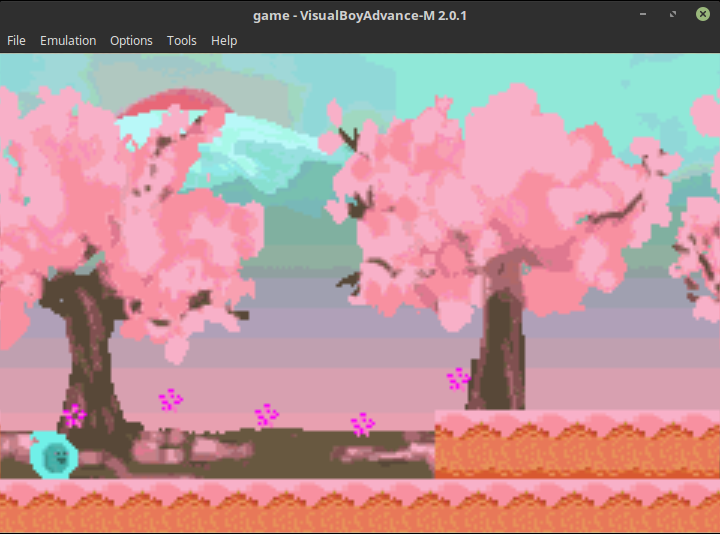
\includegraphics[width=.4\linewidth]{figuras/gba-fase5.png}
    \caption{Compara\c c\~ao da quinta fase.}%
    \label{fig:comp1}%
	\end{figure}
\end{frame}

\begin{frame}{Compara\c c\~ao entre o porte e o jogo original}
	\begin{figure}%
    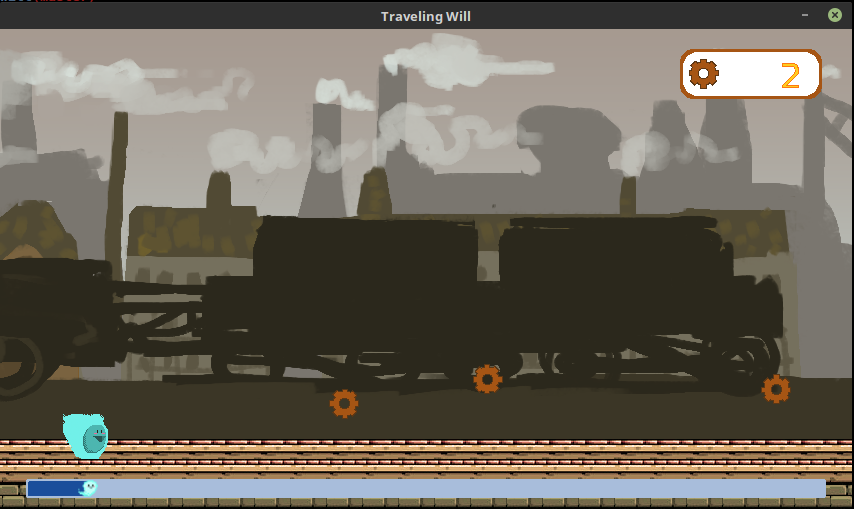
\includegraphics[width=.5\linewidth]{figuras/pc-fase6.png}
    \qquad
    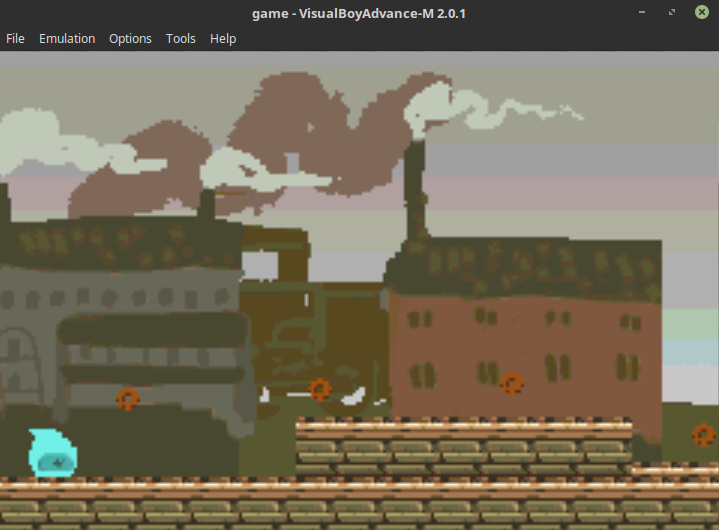
\includegraphics[width=.4\linewidth]{figuras/gba-fase6.png}
    \caption{Compara\c c\~ao da sexta fase.}%
    \label{fig:comp1}%
	\end{figure}
\end{frame}

\begin{frame}{Compara\c c\~ao entre o porte e o jogo original}
	\begin{figure}%
    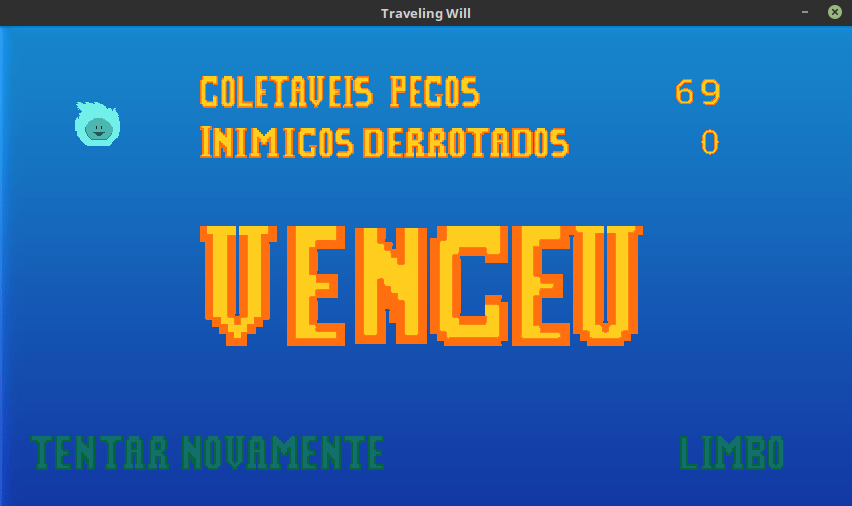
\includegraphics[width=.5\linewidth]{figuras/pc-vitoria.png}
    \qquad
    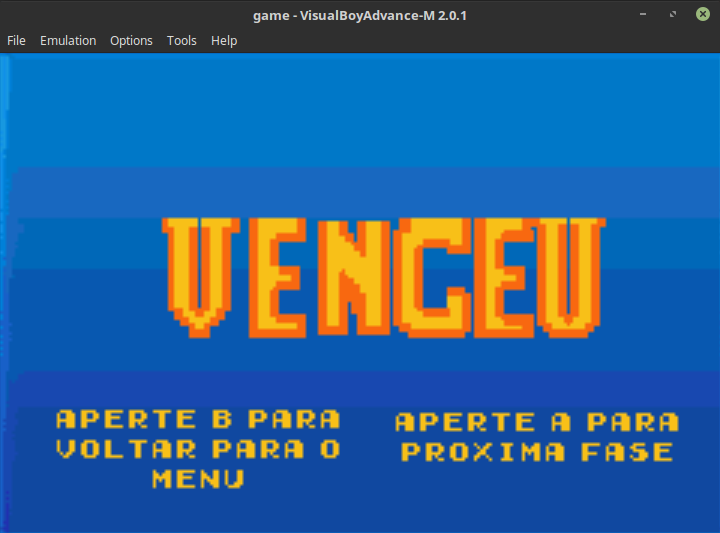
\includegraphics[width=.4\linewidth]{figuras/gba-vitoria.png}
    \caption{Compara\c c\~ao das telas de vit\'oria.}%
    \label{fig:comp1}%
	\end{figure}
\end{frame}

\begin{frame}{Compara\c c\~ao entre o porte e o jogo original}
	\begin{figure}%
    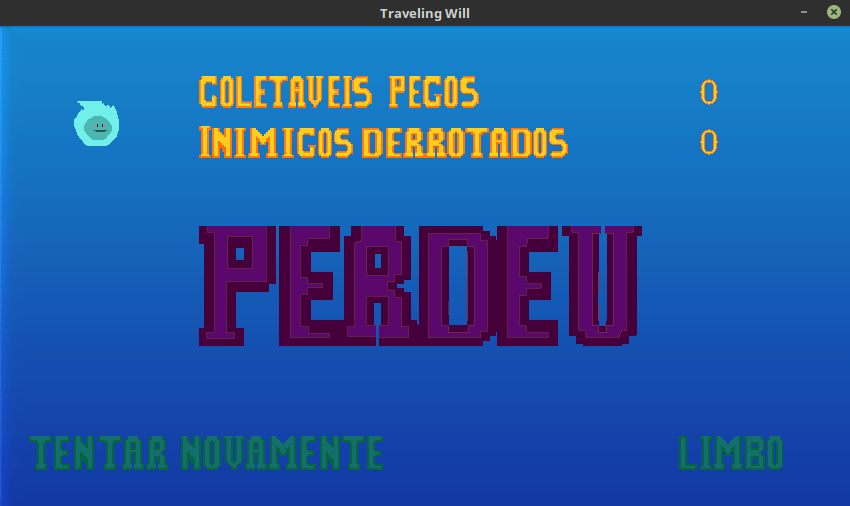
\includegraphics[width=.5\linewidth]{figuras/pc-derrota.png}
    \qquad
    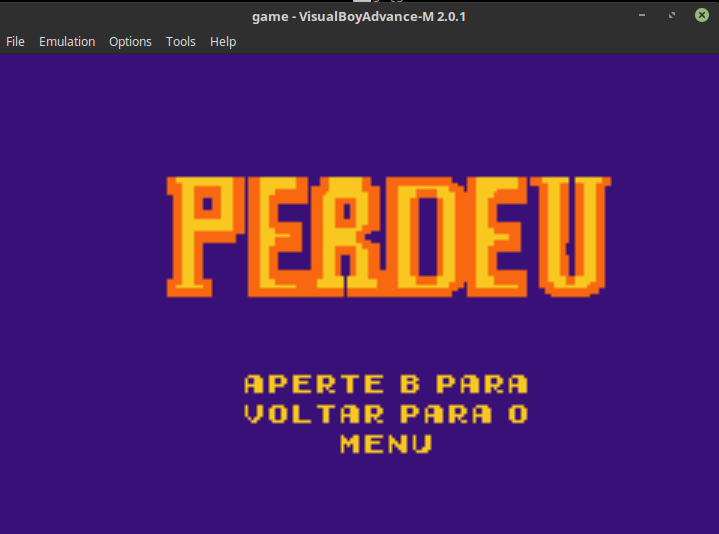
\includegraphics[width=.4\linewidth]{figuras/gba-derrota.png}
    \caption{Compara\c c\~ao das telas de derrota.}%
    \label{fig:comp1}%
	\end{figure}
\end{frame}

\section{Considera\c c\~oes Finais e Trabalhos Futuros}

\begin{frame}{Considera\c c\~oes Finais}
	Principais impedimentos durante a execu\c c\~ao do trabalho:
	\begin{itemize}[<+->]
		\item Entender detalhes do \textit{hardware do GBA};
		\item Testar o jogo no \textit{console};
		\item Adapta\c c\~ao de imagens e m\'usicas do jogo;
	\end{itemize}
\end{frame}

\begin{frame}{Considera\c c\~oes Finais}
	Pontos de melhoria p\'os-execu\c c\~ao do trabalho:
	\begin{itemize}[<+->]
		\item Melhor prioriza\c c\~ao das tarefas a serem executadas;
		\item Testes mais frequentes no \textit{console}
	\end{itemize}
\end{frame}

\begin{frame}{Considera\c c\~oes Finais}
	\textit{\'E poss\'ivel portar o jogo Traveling Will,
desenvolvido para PC pelos autores deste trabalho, para o Nintendo Gameboy Advance, no
contexto de um trabalho de conclus\~ao de curso, com performance e jogabilidade pr\'oximos
da vers\~ao para computador?}
\par
R: \textbf{Sim, \'e poss\'ivel.}
\end{frame}

\begin{frame}{Trabalhos futuros}
	\begin{itemize}[<+->]
		\item Melhorar m\'odulo de \'audio para carregar efeitos sonoros e pausar m\'usicas;
		\item Implementar carregamento e utiliza\c c\~ao de fontes;
		\item Adicionar elementos de HUD e sele\c c\~ao de fases;
		\item Salvar o estado do jogo em mem\'oria;
		\item Implementar um desfragmentador de mem\'oria na classe \texttt{MemoryManager}
	\end{itemize}
\end{frame}

\begin{frame}{Considera\c c\~oes Finais}
	Obrigado!
\end{frame}

\end{document}
